%!TEX root = ../gronskiy_phd_thesis.tex 
\chapter{Informal Introduction}

\hfill
\begin{minipage}[t]{.75\textwidth}
\textit{``Se jeunesse savoit; si viellesse pouvoit.'' \\
  (fr. ``If youth knew; if age could.'')} \\
  \hrule
  \vspace{.2cm}
  \hfill
  \textsc{--- Henri ESTIENNE}
\end{minipage}

\section{Information vs. Freedom of Choice}

When a light aircraft, while flying on a sunny day in a relatively flat area
around Langenthal in Switzerland, gets a sudden engine failure at a high
altitude, it is usually not the landing moment itself that constitutes the
difficulty~--- a well-trained pilot can land his engineless airplane anywhere,
provided some conditions are met (flatness, no major obstacles, good ground
quality). The problem of surviving an engine failure actually becomes an
optimization problem of finding the best field. And two contradictory processes
are happening at the same time: while the airplane glides down, the pilot gets
more and more information about the approaching terrain, as he sees it better
(trees, power lines, small rivers). But at the same time he ``zooms in'' closer
to the terrain, loses altitude and has fewer and fewer fields available in his
reach~(Figure~\ref{fig:airplane}).
\begin{figure}[bh!]
    \centering
    \begin{subfigure}[b]{.49\textwidth}
        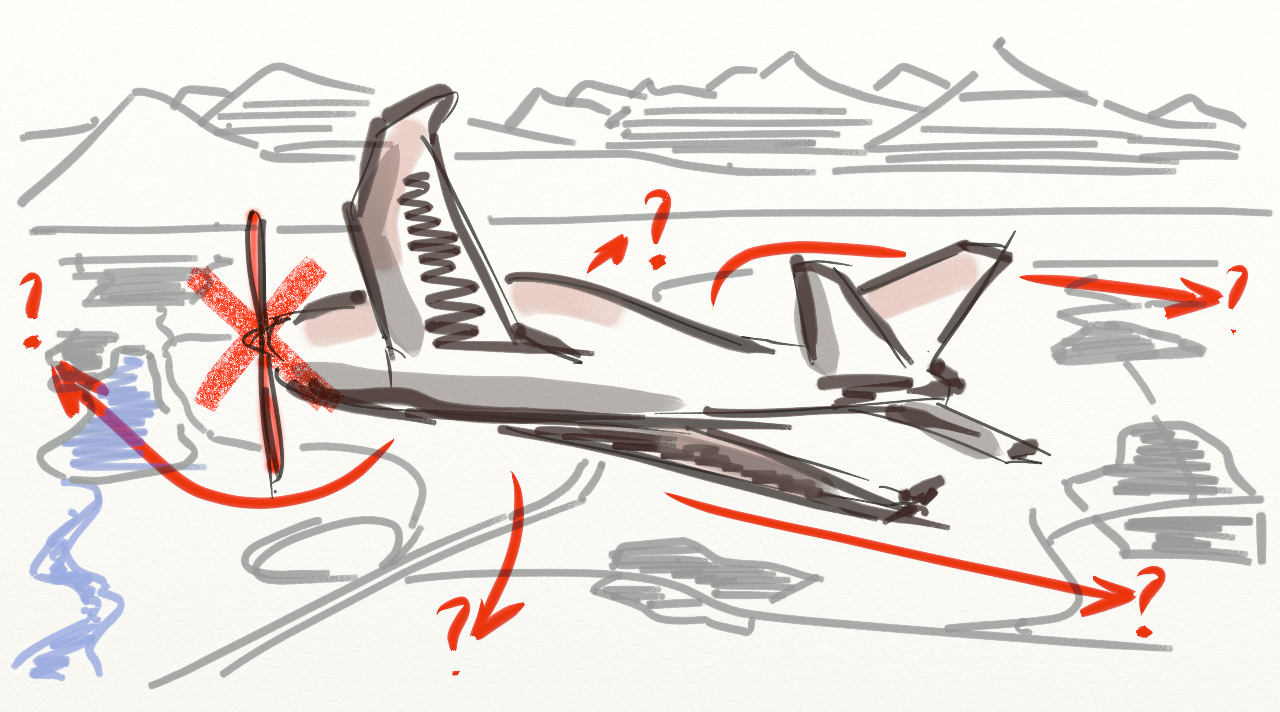
\includegraphics[width=\linewidth]{figures/ch_introduction/airplane-1}
        \caption{Little information, many choices}
        \label{fig:airplane-1}
    \end{subfigure}
    \hfill
    \begin{subfigure}[b]{.49\textwidth}            
        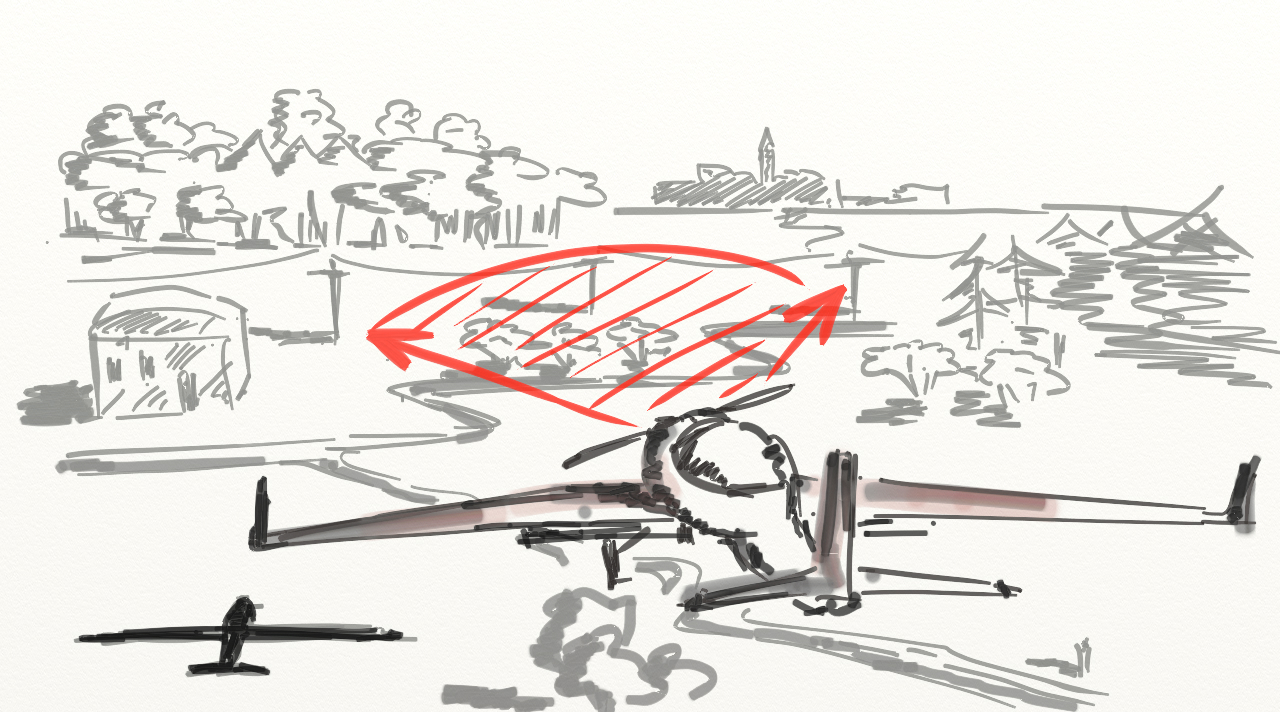
\includegraphics[width=\linewidth]{figures/ch_introduction/airplane-2}
        \caption{Much information, few choices}
        \label{fig:airplane-2}
    \end{subfigure}
    \\[.5cm]
    \caption{So much of a problem...}
    \label{fig:airplane}
\end{figure}

A field  which looks great from a high altitude can later turn out to be crossed
by a small creek with a power line on the front side, and pilot cannot climb any
more to reach ``that another nice one I've seen over that hill''. It is an
inevitable trade-off: \textit{information almost always comes at a cost of
reduced freedom of action} (hence the epigraph to this chapter). One cannot
infinitely search for the best solution and has to stop and commit at some
point. How to choose that point? A good question for a pilot.

\begin{algorithm}[b]
\caption{Prim's Algorithm for finding Minimum Spanning Tree}\label{alg:prim_intro}
\KwIn{undirected graph with non-negative weights}
\KwOut{spanning tree with minimum total weight}
{initialize current tree by choosing the first vertex randomly\;}
\While{not all vertices are in tree}{
  {find the minimal edge from current tree to the rest\;}
  {add it to the tree\;}
}
\KwRet{current tree}
\end{algorithm}

\begin{figure}[th!]
        \centering
        \begin{subfigure}[b]{.48\textwidth}
            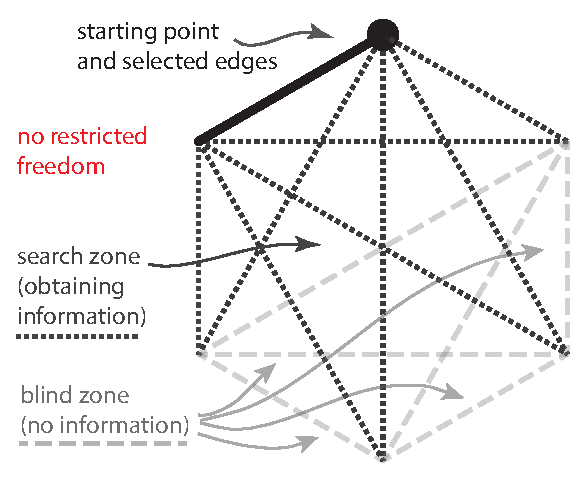
\includegraphics[width=\linewidth]{figures/ch_introduction/mst_illustration_0}
            \caption{Step 2: blind zone is large, no restricted zone yet}
            \label{fig:mst_illustration-0}
        \end{subfigure}
        \hfill
        \begin{subfigure}[b]{.48\textwidth}
            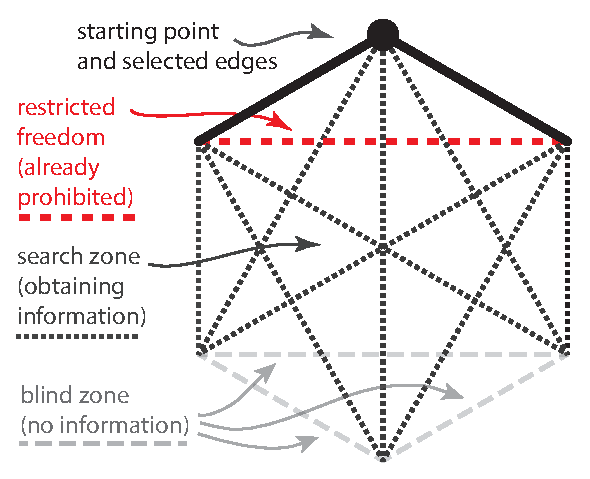
\includegraphics[width=\linewidth]{figures/ch_introduction/mst_illustration_1}
            \caption{Step 3: blind zone gets smaller, restricted zone is small}
            \label{fig:mst_illustration-1}
        \end{subfigure}
        \\[.5cm]
        \begin{subfigure}[b]{.48\textwidth}
            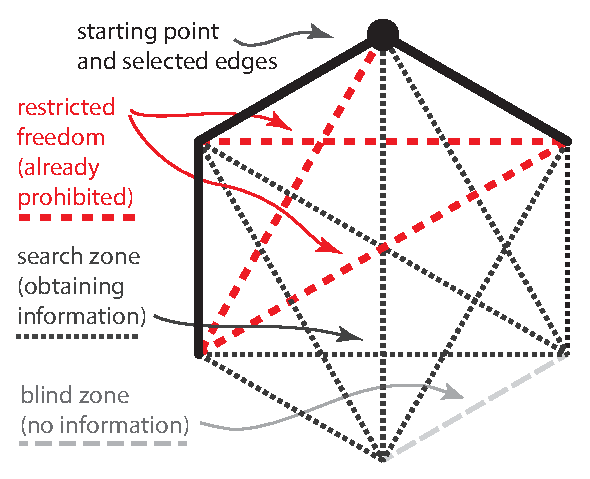
\includegraphics[width=\linewidth]{figures/ch_introduction/mst_illustration_2}
            \caption{Step 4: blind zone gets even smaller, restricted zone is growing}
            \label{fig:mst_illustration-2}
        \end{subfigure}
        \hfill
        \begin{subfigure}[b]{.48\textwidth}
            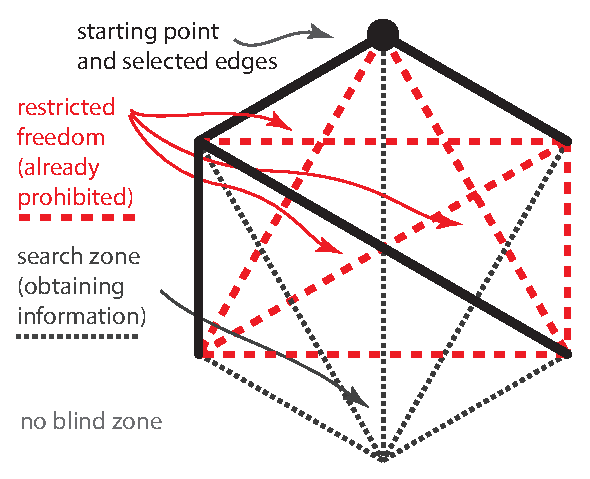
\includegraphics[width=\linewidth]{figures/ch_introduction/mst_illustration_3}
            \caption{Step 5: no blind zone vanishes, restricted zone is large}
            \label{fig:mst_illustration-3}
        \end{subfigure}
        \\[.5cm]
        \caption{Prim's MST Algorithm: freedom reduces as more of the graph is
          explored. Edge weights are not shown.}
        \label{fig:mst_illustration}
\end{figure}

But the very same question: ``when to stop (commit)?''~--- can be applied to the
field of robust algorithmic optimization. To bring an example, let us consider
some stepwise algorithm, e.g. Prim's algorithm for finding the Minimum Spanning
Tree~\citep{prim57}. \index{Minimum Spanning Tree} It will be discussed in
detail in Chapter~\ref{ch:mst}, but for now we concentrate on a simplistic
explanation of its main property~(Algorithm~\ref{alg:prim_intro}): gradually
building the optimal solution by reducing the scope of possible decisions.

\begin{table}[t!]
\centering
\begin{tabular}{p{5cm}p{5cm}}
\toprule
Pilot in trouble (Figure~\ref{fig:airplane}) & Prim's MST
(Figure~\ref{fig:mst_illustration})
\tabularnewline \midrule
    --- Pilot sees no small details of the terrain and still can literally fly
        wherever he wants.
    &
    --- On step 2, there do not yet exist any restrictions regarding which edges
        can be included into the solution, but searches through only a fraction
        of them. Blind zone is large, which yields definite lack of information.
        \tabularnewline
    --- As he descends, the pilot leaves himself less and less freedom of choice, but
    sees more and more of the details, e.g. large power-lines.
    &
    --- On step 3, the algorithm starts to create some prohibited edges,
    since no cycles are allowed. Blind zone is reducing, which reflects the fact,
    that algorithm explores more and more. \tabularnewline
    --- As he descends further, the pilot continues to lose the freedom of choice, which is yet not
    fully lost. He continues obtaining more and more details. 
    &
    --- On step 4, the algorithm continues creating prohibited edges. Blind zone is
    reduced to one edge, but still exists. \tabularnewline
    --- Finally, the pilot has no chance to divert a lot, having to land, but he now
    has a lot of information about the terrain, e.g. small creeks, trees and
    terrain roughness.
    &
    --- On step 5, the algorithm has created lots of prohibited edges, and has no
    blind zones: it basically explored all of the graph by now. \tabularnewline
\bottomrule
\end{tabular}
\caption{An analogy between real and algorithmic worlds.}
\label{table:mst_algorithm_and_pilot}
\end{table}

It is obvious that, at each further step, the Prim's algorithm: a) has fewer
possible (we call them \textit{feasible}) \index{Feasible solution} solutions
left, and b) it explores more and more detailed information
about these remaining solutions. Since ``a picture is worth a thousand words'', let's
refer to Figure~\ref{fig:mst_illustration} to illustrate this concept. The
figure brings an artificial example of four consecutive steps of Prim's MST
algorithm applied to a $6$-vertex weighted complete graph (weights are not
shown) and pays attention to three ``zones'' of edges: a ``restricted freedom''
zone (edges which will never be considered in the solution), a ``search zone''
(currently considered edges), and a ``blind zone'' (edges which are not yet
considered and thus their information does not contribute at the current step).
One can see the following:
\begin{itemize}
  \item On step 2, the algorithm still expects all edges to be feasible, but 
    searches through only a fraction of them. The blind zone is large, which yields
    definite lack of information.
  \item On step 3, the algorithm starts to create some prohibited edges,
    since no cycles are allowed in a solution. The blind zone is reducing.
  \item On step 4, the algorithm continues creating prohibited edges. The blind zone is
    reduced to one edge, but still exists.
  \item On step 5, the algorithm has created lots of prohibited edges, and has no
    blind zones: it has explored all of the graph by now.
\end{itemize}

To build a connection to the previous fictional example of the real-world
decision making, we refer to Table~\ref{table:mst_algorithm_and_pilot}. The
above property of ``increasing information and reducing freedom'' is
characteristic to many algorithms and, more generally, to systems where the
notion of ``being optimal'' is defined. 

But why are we talking about that? Because having all the possible information
sometimes does not help to select the best solution, as well as having all the
freedom to choose solutions sometimes fails~--- there exists an
\textit{informativeness vs. robustness trade-off}. \index{Trade-off}
\index{Trade-off!Informativeness} \index{Trade-off!Robustness} We revisit this
statement in the next section.

\section{Overly Informed Decisions Are Bad}

Information can be evil under some circumstances. To see that, revisit the
case of Prim's MST Algorithm (Figure~\ref{fig:mst_illustration} and
Algorithm~\ref{alg:prim_intro}): one can easily prove that despite all the fancy
reasoning above, Prim's algorithm always \textit{finds the optimal tree}. Why are
then all the explanations of the previous section important?

The answer is that this optimal tree is only optimal in current instance of
graph weights, which most likely contain \textit{noise}. In fact, all the
real-world observations are contaminated by noise, making it impossible to judge
truth without uncertainty. In terms of our two examples, a very informal
Table~\ref{table:mst_algorithm_and_pilot_noise} explains the analogy. In fact,
it turns out, that in presence of uncertainty, overly informative environments
can deceive the algorithm and lure it into a solution, which is, although
optimal in current instance of noise, still far from being optimal in some 
ground truth, noise-free instance.

\begin{table}[t]
\centering
\begin{tabular}{p{5cm}p{5cm}}
\toprule
Pilot in trouble (Figure~\ref{fig:airplane}) & Prim's MST
(Figure~\ref{fig:mst_illustration})
\tabularnewline \midrule
    --- At each altitude, the pilot sees not all the details
    because there are limitations to his vision (or visibility).
    &
    --- At each step, the algorithm observes noised weights of edges, i.e.~some
    randomness exists.
    \tabularnewline
    --- As a consequence, certain decisions can eliminate possibilities to land
    on fields which seem bad from current altitude but in fact are the best.
    &
    --- As a consequence, certain decisions can eliminate edges which seem
    bad in the current instance, but are very good on the average.
    \tabularnewline
\bottomrule
\end{tabular}
\caption{Noise in real and algorithmic worlds.}
\label{table:mst_algorithm_and_pilot_noise}
\end{table}

Intuitive (we will come to that in a more formal Chapter~\ref{ch:gen_appch})
reasoning for this phenomena of overfitting \index{Overfitting} is as follows:
an agent (pilot, algorithm) uses information contained in the environment to
solve the task. While this information contains a useful component, it keeps a
bit\footnote{``Bit'' here is not the Shannon's information-theoretic bit yet. We
come to it later.} of noise-induced ``garbage''. Filtering the latter out is thus the
key to decent performance. There is a group of methods called
\textit{regularization} \index{Regularization} to fulfill this task.

\section{Regularization by Stochastic Approximation}

While there are lots and lots of ways to regularize solutions to various
optimization problems, we will start the story of this thesis from a point which
we already touched above: approximating solutions. This concept will be central
to the first three chapters of the thesis, leading to surprising conjectures in
the last chapter.

But first things first: informally speaking, stochastic approximation allows us
to avoid optimizing the given objective till the global minimum~--- remember
from above that this global minimum might be not the best one in
expectation!~--- but instead \textit{stops} optimizing at some moment before the
end, leaving us some room near the optimum to choose from. In most cases, one
will then choose randomly from a set of these near-optimal solutions, called an
\textit{approximation set}.

\myremark Revisiting the above example of our pilot for the last time (and let
him land safely), this means: make him descend to some predefined altitude $h >
0$ (it can be low, but not zero), and then stop his (no longer reliable)
cognitive process, choose a field randomly from the \textit{approximation set}
of nearby fields and commit to landing on that one.
\index{Approximation set}

We now would like to make a small side-leap and connect the above approximation
intuition with the field of statistical physics. An important observation is to
note that Mother Nature essentially does the same stochastic approximation when
optimizing energy of states in large particle systems. This phenomenon is
largely studied in, for example, statistical mechanics. In fact, real systems
never find the global optimum of energy, but sample their states from some
distribution (sometimes called~\textit{Gibbs distribution}), which
\textit{concentrates} around optimal states, but assigns some probability to
near-optimal states.
\index{Gibbs distribution}

\begin{figure}[t]
    \centering
    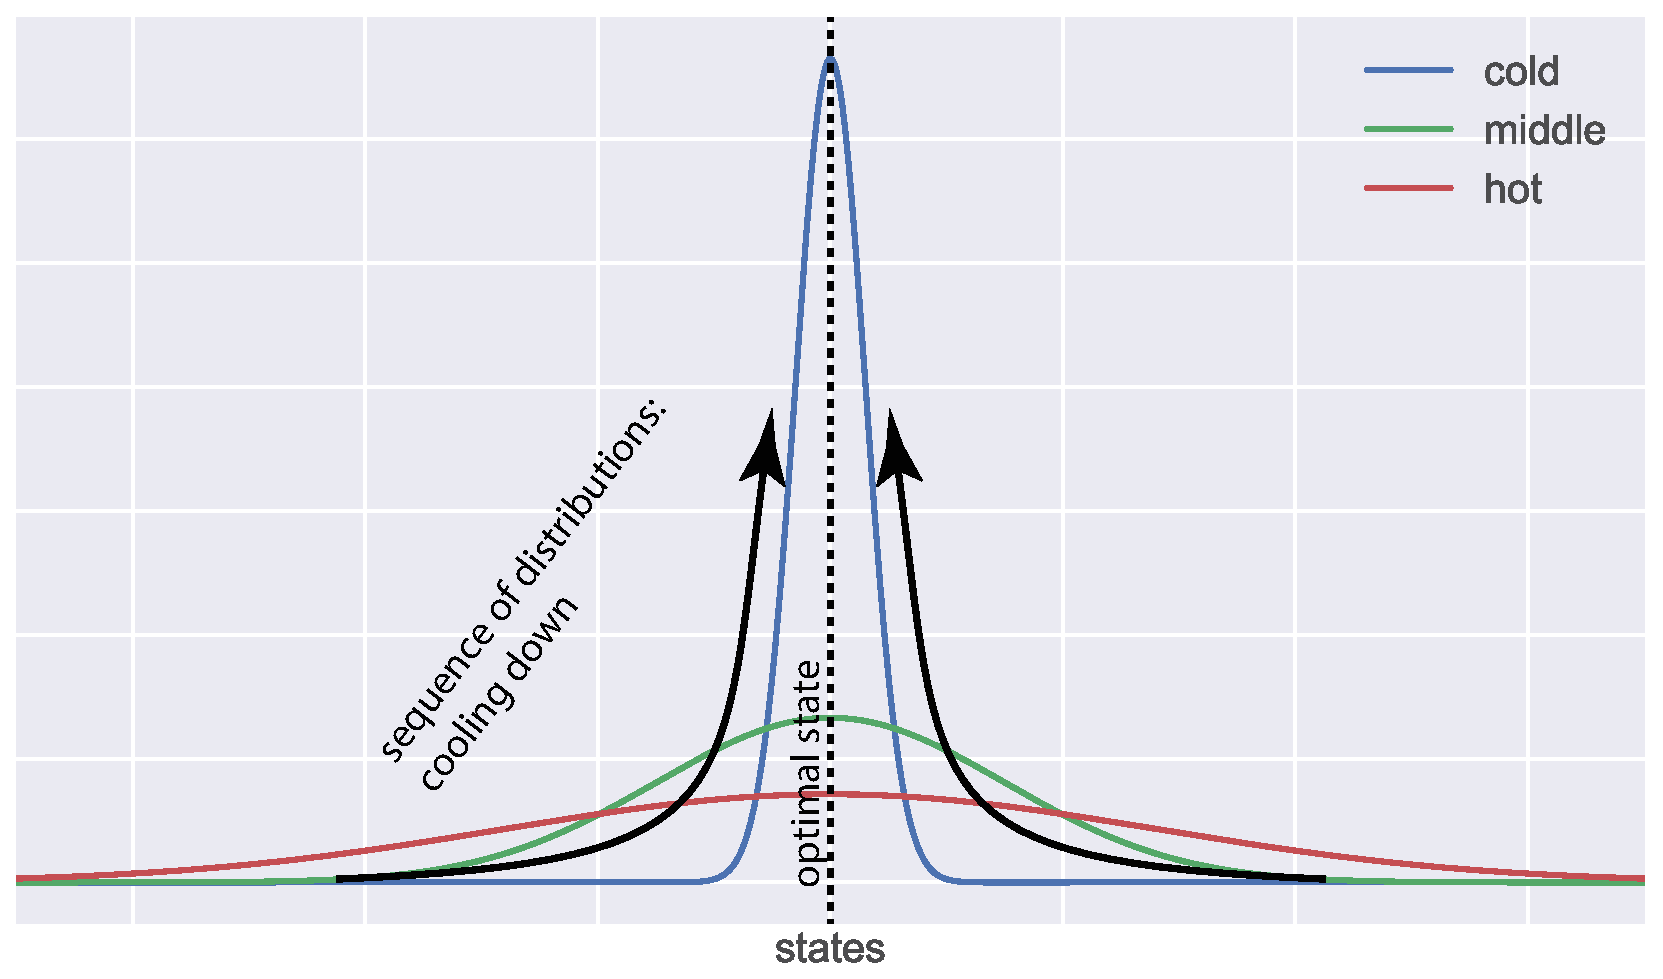
\includegraphics[width=.8\textwidth]{figures/ch_introduction/gibbs_cooling}
    \\[.5cm]
    \caption{Sequence of Gibbs distributions as temperature decreases (``cooling down'')}
    \label{fig:introduction_gibbs_cooling}
\end{figure}

In fact, what we call \textit{temperature} is exactly the parameter which
controls how closely the sampled states approximate the optimal state: an H$_2$O
molecule of water steam at $120$~C$^\circ$ has more freedom to move around than
a molecule of water liquid at $40$~C$^\circ$, which in turn still has more
freedom than a molecule of frozen ice at $-40$~C$^\circ$. This concept is
illustrated by Figure~\ref{fig:introduction_gibbs_cooling}, in which case
temperature is the ``width'' of distribution.

While the idea of approximate solutions is, of course, not new, the cornerstone of
the thesis is to offer a novel answer to the question on \textit{how to choose}
the level of approximation, at which one should sample to obtain robust
solutions. Throughout the thesis, we will formulate this question and answer it from
several prospectives, which we explain in the next section.

\section{Thesis Contributions and Outline}

Precise objectives and contributions are stated separately in each chapter.
Here, we describe them in a survey manner.
\begin{itemize}
    \item {\sffamily\bfseries (Chapter~\ref{ch:gen_appch})}
    To start, we revisit an approximate set-based approach to robust solving, called
    \textit{Approximation Set Coding}. We provide its theoretical background. We
    then introduce and experimentally evaluate an abstract, but still
    interpretable proof-of-concept model, and show the superiority of the
    approximation set-based approach in terms of error. However, this approach
    involves a computationally expensive step. To address it, we prove a
    theoretical result which partially solves the computational bottleneck
    problem. We provide experiments for that as well.
    \item {\sffamily\bfseries (Chapter~\ref{ch:mst})}
    As an expansion of the above approach, we adapt and apply it in algorithmic
    setting, specifically for algorithms which solve the Minimum Spanning Tree
    problem. We show that the approach allows us not only to robustly solve such
    problems, but also ranks various algorithms according to their robustness.
    Finally, our algorithmic adaptation is free of the computational bottleneck
    exhibited in the general setting.
    \item {\sffamily\bfseries (Chapter~\ref{ch:free_energy})} 
    Further, we study a thermodynamical Gibbs relaxation of the approximation
    set-based approach in combinatorial optimization setting and discover its
    deep connection with a prominent task in statistical mechanics, namely
    the task of computing the \textit{free energy density} (for definition
    and details, refer to the respective chapter). The contribution is thus
    twofold: first, we devise and apply the Gibbs relaxation of approximation
    set-based approach, and second, we prove a mathematical result associated
    with it, which has its own importance.
    \item {\sffamily\bfseries (Chapter~\ref{ch:smbp_and_rem})}
    In the last chapter, we drift away from the approximating solutions.
    Inspired by the theoretical results of the previous chapter, we ask
    fundamental questions about statistical mechanics of combinatorial
    optimization and how it defines our ability to efficiently solve them. We
    pick a combinatorial optimization problem and compare its \textit{large
    system size} behavior with the one of well-known Random Energy Model (REM),
    leading to some interesting conjectures about search complexity.
\end{itemize}

Final notes and possible directions of further work are discussed in
Chapter~\ref{ch:conclusion}.

\section{Statement of Publications and Joint Contributions}

\subsection*{Publications}

The following publications appeared while working on this thesis, or were under
review by the time of completing this thesis. I was either the main contributor
or jointly contributing with my co-authors:
\begin{itemize}
    \item \citep{gronskiy14} \\
    \textbf{Gronskiy, A.}, Buhmann, J. M., 2014. How informative are minimum
    spanning tree algorithms? In: 2014 IEEE International Symposium on
    Information Theory (ISIT) 2014;

    \item \citep{aofa2014} \\
    Buhmann, J. M., \textbf{Gronskiy, A.}, Szpankowski, W., 2014. Free energy rates
    for a class of very noisy optimization problems. In: Analysis of Algorithms
    (AofA) 2014;

    \item \citep{analco17} \\
    Buhmann, J. M., Dumazert, J., \textbf{Gronskiy, A.}, Szpankowski, W., 2017b. Phase
    transitions in parameter rich optimization problems. In: Proceedings of
    the Fourteenth Workshop on Analytic Algorithmics and Combinatorics, ANALCO
    2017;

    \item \citep{jcss:2017} \\
    Buhmann, J., \textbf{Gronskiy, A.}, Mihal\'ak, M., Pr\"oger, T.,
    \v{S}r\'amek, R., Widmayer, P., 2017. Robust optimization in the presence of
    uncertainty: A generic approach. Journal of Computer and System Sciences.

    \item (under review) \\
    \textbf{Gronskiy, A.}, Buhmann, J. M., Szpankowski, W., 2018. Free Energy Asymptotics
    for Problems with Weak Solution Dependencies. In: 2018 IEEE International
    Symposium on Information Theory (ISIT) 2018;

    \item (under review) \\
    Buhmann, J. M., Dumazert, J., \textbf{Gronskiy, A.}, Szpankowski, W., 2018.
    Posterior Agreement for Large Parameter-Rich Optimization Problems. In:
    Journal of Theoretical Computer Science.
\end{itemize}

The following publication is aligned with the topic of the thesis, however I 
did not contribute to it significantly:
\begin{itemize}
    \item \citep{bian16} \\
    Bian, Y., \textbf{Gronskiy, A.}, Buhmann, J. M., 2016. Information-theoretic analysis
    of max-cut algorithms. In: 2016 Information Theory and Applications
    Workshop, (ITW), 2016.
\end{itemize}

The following Master's theses were completed under my advisorship:
\begin{itemize}
    \item Dumazert, J., 2015. Free Energy for a Class of Combinatorial
    Optimization Problems and its Asymptotics. ETH Zurich;
    \item Negulescu, G., 2015. Theoretical and Numerical Analysis of an
    Information-Theoretic Approach to Feature Selection. ETH Zurich;
    \item Gence, E., 2017. Electrocardiogram Feature Extraction for Takotsubo
    Syndrome Detection. ETH Zurich (I acted as co-advisor).
\end{itemize}

\subsection*{Joint Contributions}

The ideas in this thesis were mostly developed by me, but some of them were
developed jointly with collaborators. Here, I identify major collaborations and
contributions which are not due to me. For detailed statements of contributions
and notes on presentation, see introductions to the respective chapters
(Sections~\ref{sec:asc_contribs}, \ref{sec:mst_contribs},
\ref{sec:free_energy_contribs} and \ref{sec:smbp_and_rem_contribs}).

\begin{itemize}
    \item {\sffamily\bfseries (Chapter~\ref{ch:gen_appch})}
    The ASC approach~\citep{conf/isit/Buhmann10} and Similarity
    approach~\citep{Sramek:PhD} served as a starting point for this
    thesis, explained in Sections~\ref{sec:asc_original}
    and~\ref{sec:similarity_approach_intro} respectively. We devised the
    proof-of-concept model of Section~\ref{sec:proof_of_concept} jointly with
    T.~Pr\"oger, but he implemented the vast majority of the experiments.
    Theorem~\ref{thm:oracle_similarity} is my contribution.
    \item {\sffamily\bfseries (Chapter~\ref{ch:mst})}
    Contributions, design and implementation are fully due to me.
    \item {\sffamily\bfseries (Chapter~\ref{ch:free_energy})} 
    This was a joint work with W.~Szpankowski and, partially, with J.~Dumazert.
    Contributions are mainly due to me. The main idea behind proof of
    Theorem~\ref{thm:lawler_qap_tight_bound} is due to J.~Dumazert.
    \item {\sffamily\bfseries (Chapter~\ref{ch:smbp_and_rem})}
    Contributions are fully due to me.
\end{itemize}


In general, I appreciate all
the inputs I have ever obtained. It is hard to extract which specific bit comes
from whom, because most of theoretical work was accompanied by lots of
discussions, e-mail exchanges, marker-and-whiteboard as well as
chalk-and-blackboard sessions or coffee brainstorming with lots of people
to whom I am incredibly grateful.


